\documentclass{beamer}

\usepackage[utf8]{inputenc}

\setbeamercovered{transparent}
\setbeamertemplate{navigation symbols}

\setbeamertemplate{footline}{\makebox[0.98\paperwidth][r]{\large \raisebox{1.2ex}{\insertframenumber}}}

\title{DNSKEY Management}

\author{Julien Perrochet \and Tobias Schlatter}
\date{December 12, 2012}
\institute{ITSEC, EPFL, Prof. Janson}

\graphicspath{{../figures/}}

\begin{document}

\begin{frame}
  \titlepage
\end{frame}

\section{Outline}
\begin{frame}
  \frametitle{Outline}

  \begin{block}{Introduction}
  \end{block}

  \begin{block}{Current DNSSEC Deployment}
  \end{block}

  \begin{block}{DNSKEY Management}
  \end{block}

  \begin{block}{Case-Study: Switzerland}
  \end{block}

\end{frame}

\section{Introduction}
\begin{frame}
  \frametitle{DNSSEC Chain of Trust}

  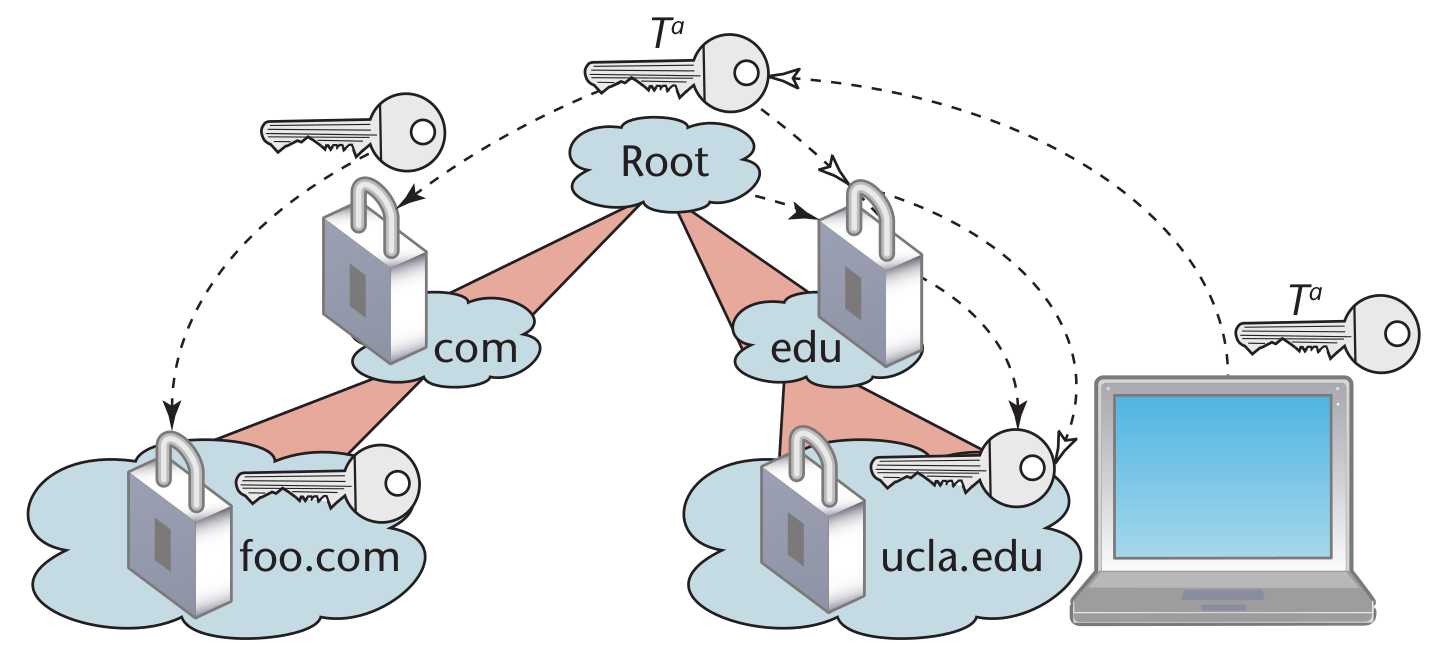
\includegraphics[width=\textwidth]{trust-chain}

\end{frame}

\begin{frame}
  \frametitle{Relevant Operations}

  \begin{block}{Foo}

  \end{block}

\end{frame}

\section{DNSSEC Deployment}

\begin{frame}
  \frametitle{DNSSEC Production Zones}
  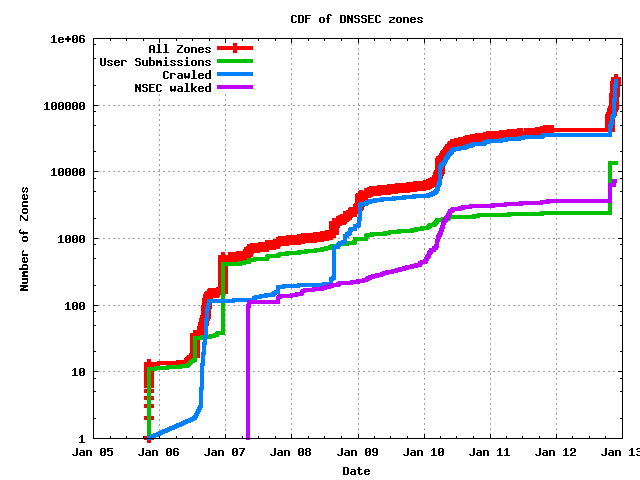
\includegraphics[width=\textwidth]{dnssec-growth}
\end{frame}

\begin{frame}
  \frametitle{DNSSEC Certificate Chain}
  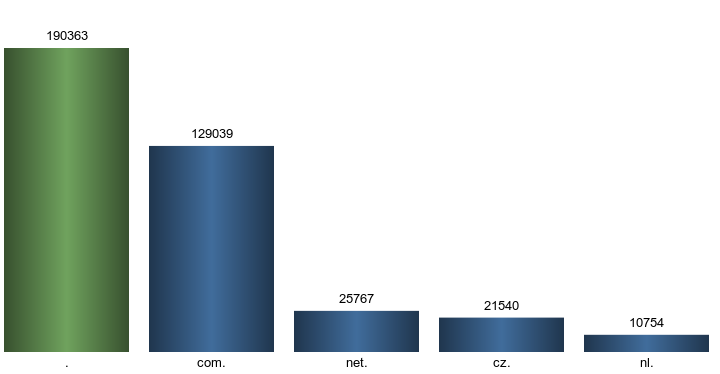
\includegraphics[width=\textwidth]{dnssec-on-tlds}

  %% Mention TARs
\end{frame}

\section{Operations}

%% TODO

\section{Case-Study: CH}


\end{document}

%%% Local Variables: 
%%% mode: latex
%%% TeX-master: t
%%% End: 
